%%%%%%%%%%%%%%%%%%%%%%%%%%%%%%%%%%%%%%%%%
% Adapted from the template available at https://www.latextemplates.com/template/jacobs-landscape-poster
%
%%%%%%%%%%%%%%%%%%%%%%%%%%%%%%%%%%%%%%%%%

%----------------------------------------------------------------------------------------
%	PACKAGES AND OTHER DOCUMENT CONFIGURATIONS
%----------------------------------------------------------------------------------------

\documentclass[final]{beamer}

    \usepackage[scale=1.24]{beamerposter} % Use the beamerposter package for laying out the poster
    
    \usepackage{anyfontsize}
    \usepackage{fontspec}
    \usepackage[T1]{fontenc}
    \DeclareTextCommand{\nobreakspace}{T1}{\leavevmode\nobreak\ }
    \usepackage{setspace}
    
    \usetheme{confposter} % Use the confposter theme supplied with this template

    % Many more colors are available for use in beamerthemeconfposter.sty
    
    % Define the column widths and overall poster size
    % To set effective sepwid, onecolwid and twocolwid values, first choose how many columns you want and how much separation you want between columns
    % In this template, the separation width chosen is 0.024 of the paper width and a 4-column layout
    % onecolwid should therefore be (1-(# of columns+1)*sepwid)/# of columns e.g. (1-(4+1)*0.024)/4 = 0.22
    % Set twocolwid to be (2*onecolwid)+sepwid = 0.464
    % Set threecolwid to be (3*onecolwid)+2*sepwid = 0.708
    
    \newlength{\sepwid}
    \newlength{\onecolwid}
    \newlength{\twocolwid}
    \newlength{\threecolwid}
    \setlength{\paperwidth}{48in} % A0 width: 46.8in
    \setlength{\paperheight}{36in} % A0 height: 33.1in
    \setlength{\sepwid}{0.024\paperwidth} % Separation width (white space) between columns
    \setlength{\onecolwid}{0.22\paperwidth} % Width of one column
    \setlength{\twocolwid}{0.464\paperwidth} % Width of two columns
    \setlength{\threecolwid}{0.708\paperwidth} % Width of three columns
    \setlength{\topmargin}{-0.5in} % Reduce the top margin size
    %-----------------------------------------------------------
    
    \usepackage{graphicx}  % Required for including images
    
    \usepackage{booktabs} % Top and bottom rules for tables
    
    %----------------------------------------------------------------------------------------
    %	TITLE SECTION 
    %----------------------------------------------------------------------------------------
    
    \title{Effective Visualization of Sparse Machine Learning Results Applied to Brain Imaging Modalities Derived from the TADPOLE Challenge \\[0.5in]} % Poster title
    
    \author{Zoe Baker \& Madeline McKune  Advised by Dr. Hua Wang \& Lodewijk Brand} % Author(s)
    
    \institute{Computer Science Department\\Colorado School of Mines} % Institution(s)
    
    %----------------------------------------------------------------------------------------
    
    \begin{document}
    
    \addtobeamertemplate{block end}{}{\vspace*{2ex}} % White space under blocks
    \addtobeamertemplate{block alerted end}{}{\vspace*{2ex}} % White space under highlighted (alert) blocks
    
    \setlength{\belowcaptionskip}{2ex} % White space under figures
    \setlength\belowdisplayshortskip{2ex} % White space under equations
    
    \begin{frame}[t] % The whole poster is enclosed in one beamer frame
    
    \begin{columns}[t] % The whole poster consists of three major columns, the second of which is split into two columns twice - the [t] option aligns each column's content to the top
    
    \begin{column}{\sepwid}\end{column} % Empty spacer column
    
    \begin{column}{\onecolwid} % The first column
    
        %----------------------------------------------------------------------------------------
        %	MOTIVATION
        %----------------------------------------------------------------------------------------
        
        % Optional starting image
        % \begin{center}
        %     
\includegraphics[width=\linewidth]{images/placeholder.jpg}
        % \end{center}

        \begin{alertblock}{Motivation}
        
            \textbf{MRI and PET scans are commonly used for diagnosing Alzheimer’s disease (AD) because they are non-invasive and widely available}. These scans can show brain atrophies that are solidly linked to cognitive decline and help physicians make an accurate diagnosis. Researchers run machine learning algorithms on MRI and PET scans to isolate regions of interest (ROI) in the brain most associated with an Alzheimer’s disease diagnosis. Taking this brain data and effectively visualizing it is important for interpreting results and seeing if machine learning results contradict or confirm prior medical understanding. Visualizations also bridge the gap between the medical communities and the public by making the data easier to understand. For example, hearing that a region of the brain is affected vs seeing that region, or related regions of the brain, is “lit up”. Brain visualizations allow for quick and effective communication of the results of machine learning algorithms.
            \vspace{2cm}
            \begin{figure}
                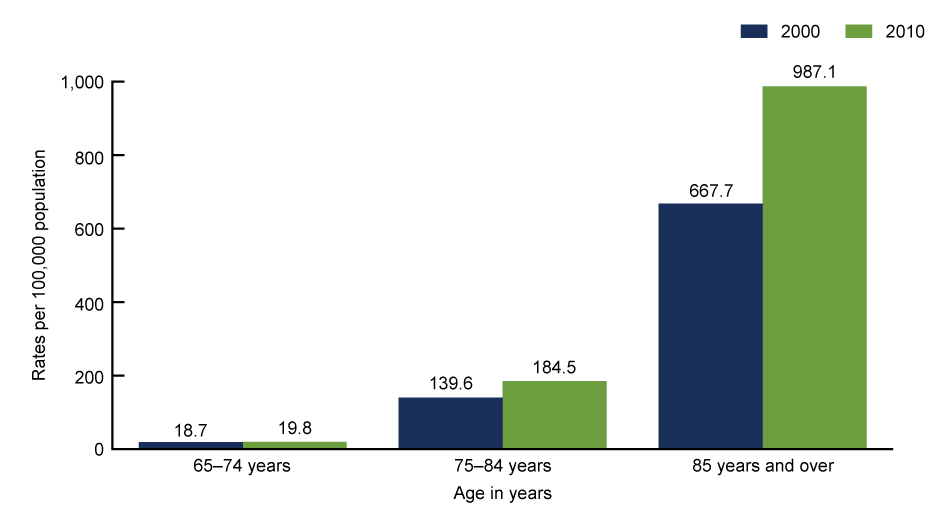
\includegraphics[width=1.0\textwidth,keepaspectratio]{images/alzRate.PNG}
                \vspace{1cm}
                \caption{Age-Adjusted Death Rates for Alzheimer's Disease: United States 2000 and 2010}\label{imageLabel}
           \end{figure}
           \vspace{1cm}
        
        \end{alertblock}
        
        

        %----------------------------------------------------------------------------------------
        %	METHODS
        %----------------------------------------------------------------------------------------
        
       % \begin{block}{Title}
        %
         %   Commodo exercitation ex nostrud ullamco elit cillum et est aliqua eu eu. Ut eu laborum tempor tempor eiusmod aute eu aute. Aute dolore nisi in sunt do enim tempor aliquip non consequat ut nisi consectetur pariatur. Ullamco sint ex enim aute tempor ad laborum nulla adipisicing dolore proident elit. Eu fugiat reprehenderit et pariatur id adipisicing anim minim veniam enim aliqua laborum. \\[0.3in]
            

          %  \begin{figure}
           %     
\includegraphics[width=0.8\textwidth,keepaspectratio]{images/placeholder.jpg}
            %    \caption{Caption}
        %    \end{figure}
        
    %    \end{block}
        
        %----------------------------------------------------------------------------------------
    
    \end{column} % End of the first column
    
    \begin{column}{\sepwid}\end{column} % Empty spacer column
    
    \begin{column}{\twocolwid} % Begin a column which is two columns wide (column 2)
    
       \begin{alertblock}{Methods}
        
            \textbf{The Nilearn module requires a brain atlas and a weight matrix to plot brain imaging data.} A brain atlas is set of coordinates that define a region in the brain correlated with a certain function: speech, movement, memory, etc. The ROIs from the TADPOLE dataset were fit so they correlated to a predefined Nilearn region with the help of built-in Nilearn functions. Then the calculated multivariate linear regression (XW=y) for a specific ROI can be matched to an atlas.The ROI measurements are normalized from 0-1, representing their weight or “intensity”. These weights were fed into Nilearn in the order of the brain atlas so that the ROIs are mapped with their corresponding intensity. The Glass Brain module from Nilearn represents white/yellow regions as low intensity and red/black regions as high intensity.   
            \linebreak
            \linebreak Potentially: A machine learning algorithm could be run on MRI and PET brain volume data, associating each ROI with a particular weight that corresponds to its correlation with an Alzheimer’s diagnosis. This w-vector could then be plotted on a brain to highlight the ROIs most important to consider when making an Alzheimer’s diagnosis. 
        \end{alertblock}
        
    %    \begin{block}{Title}
        
     %       Potentially: A machine learning algorithm could be run on MRI and PET brain volume data, associating each ROI with a particular weight that corresponds to its correlation with an Alzheimer’s diagnosis. This w-vector could then be plotted on a brain to highlight the ROIs most important to consider when making an Alzheimer’s diagnosis. 

            %\begin{itemize}
             %   \item Item 1
              %  \item Item 2
               % \item Item 3
                %\item Item 4
            %\end{itemize}

    %    \end{block}


    %----------------------------------------------------------------------------------------
    %	OUR IMAGES
    %----------------------------------------------------------------------------------------

    \begin{columns}[t,totalwidth=\twocolwid] % Split up the two columns wide column again
    
        \begin{column}{\onecolwid} % The first column within column 2 (column 2.1)
        
            %----------------------------------------------------------------------------------------
            %	MRI
            %----------------------------------------------------------------------------------------
            
            \begin{block}{MRI}
            %\begin{block}
                    
                %Description of MRI \\[0.1in]
            
            \begin{figure}
                    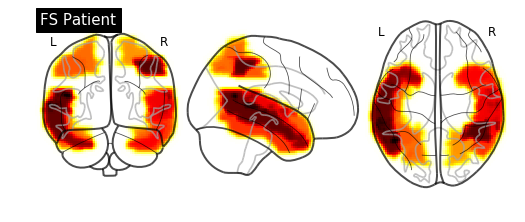
\includegraphics[width=1.0\linewidth]{images/exampleROI.png}
                    \caption{Example of plotting a region of MRI ROIs}
            \end{figure}\
         
            \begin{figure}
                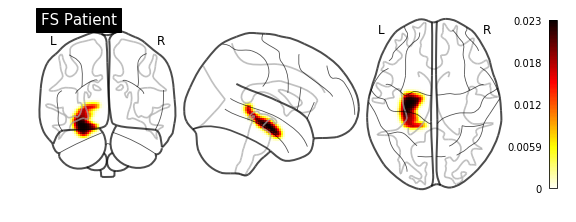
\includegraphics[width=1.0\linewidth]{images/hippo.png}
                \caption{Example of plotting the Left Hippocampus}
            \end{figure}
            \end{block}
            
            %----------------------------------------------------------------------------------------
        
        \end{column} % End of column 2.1
        
        \begin{column}{\onecolwid} % The second column within column 2 (column 2.2)
        
            %----------------------------------------------------------------------------------------
            %	PET
            %----------------------------------------------------------------------------------------
            
            \begin{block}{PET}
            %\begin{block}
            
                %Description of PET \\[0.1in]
                
                \begin{figure}
                    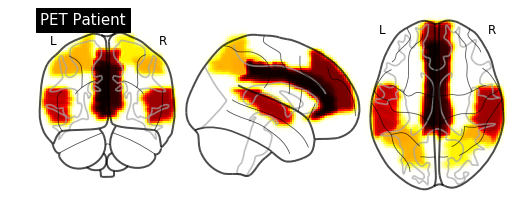
\includegraphics[width=1.0\linewidth]{images/petROI.png}
                    \caption{Example of plotting a region of PET ROIs}
                \end{figure}
                \begin{figure}
                    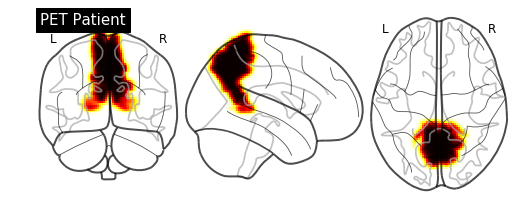
\includegraphics[width=1.0\linewidth]{images/precun.png}
                    \caption{Example of plotting the Precuneus}
                \end{figure}

            \end{block}
            
            %----------------------------------------------------------------------------------------
        
        \end{column} % End of column 2.2
    
    \end{columns} % End of the split of column 2
    
    \end{column} % End of the second column
    
    \begin{column}{\sepwid}\end{column} % Empty spacer column
    
    \begin{column}{\onecolwid} % The third column
    
    %---------------------------------------------------------------------------------------
    % METHODS IMAGE
    %------------------------------------------------------------------------------------------
     \begin{figure}
        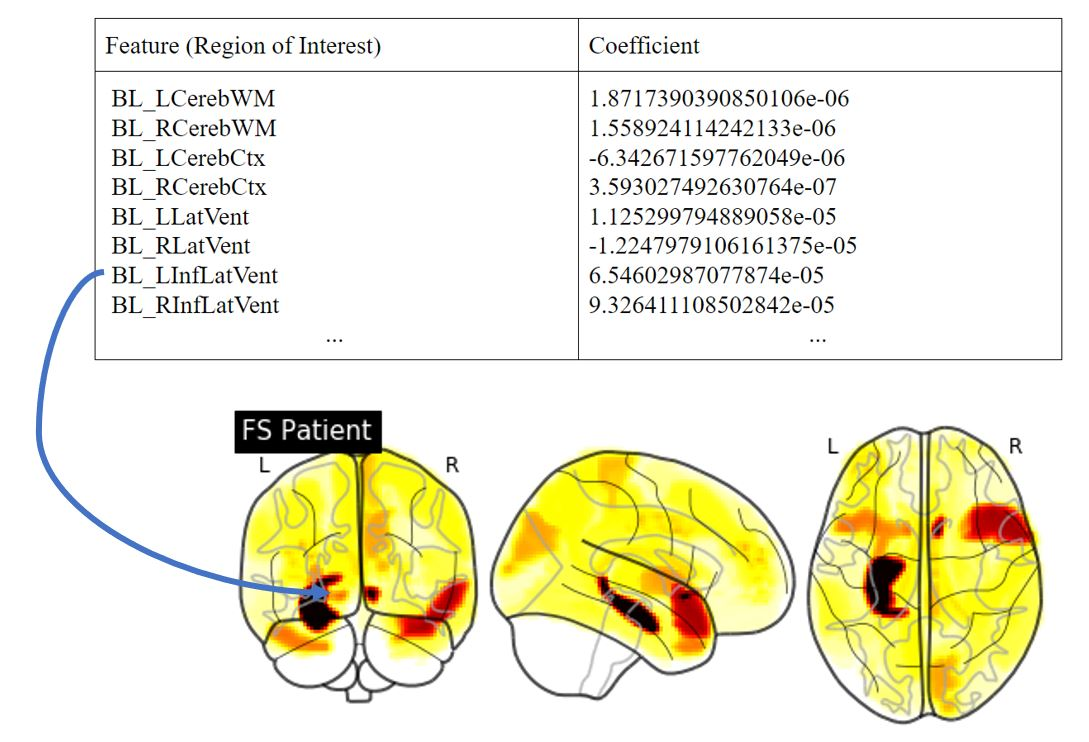
\includegraphics[width=1.0\linewidth]{images/mult.JPG}
    \end{figure}
    %----------------------------------------------------------------------------------------
    %	SUMMARY
    %----------------------------------------------------------------------------------------
    
    \begin{alertblock}{Summary}
    
        Use of the Nilearn module for plotting brain imaging data can quickly and effectively show the results of a machine learning algorithm. With Nilearn, one can easily highlight general regions of importance and see if machine learning results contradict or confirm prior medical understanding.
    
    \end{alertblock} 
    
        % %----------------------------------------------------------------------------------------
        % %	ADDITIONAL INFORMATION
        % %----------------------------------------------------------------------------------------
        
        % \begin{block}{Additional Information}
        
        % Maecenas ultricies feugiat velit non mattis. Fusce tempus arcu id ligula varius dictum. 
        % \begin{itemize}
        % \item Curabitur pellentesque dignissim
        % \item Eu facilisis est tempus quis
        % \item Duis porta consequat lorem
        % \end{itemize}
        
        % \end{block}
        
        %----------------------------------------------------------------------------------------
        %	REFERENCES
        %----------------------------------------------------------------------------------------
        
        \begin{block}{References}
        
        % \nocite{*} % Insert publications even if they are not cited in the poster
        {
            \bibliographystyle{IEEEtran}
            \scriptsize
            \bibliography{references}\vspace{0.1in}
            \linebreak
            \linebreak Abraham A, Pedregosa F, Eickenberg M, Gervais P, Mueller A, Kossaifi J, Gramfort A, Thirion B and Varoquaux G (2014) Machine learning for neuroimaging with scikit-learn. Front. Neuroinform. 8:14. doi: 10.3389/fninf.2014.00014
            \linebreak
            \linebreak Brand L. et al. (2018) Joint High-Order Multi-Task Feature Learning to Predict the Progression of Alzheimer’s Disease. In: Frangi A., Schnabel J., Davatzikos C., Alberola-López C., Fichtinger G. (eds) Medical Image Computing and Computer Assisted Intervention – MICCAI 2018. MICCAI 2018. Lecture Notes in Computer Science, vol 11070. Springer, Cham
            \linebreak
            \linebreak TADPOLE Challenge: Prediction of Longitudinal Evolution in Alzheimer's Disease, Razvan V. Marinescu, Neil P. Oxtoby, Alexandra L. Young, Esther E. Bron, Arthur W. Toga, Michael W. Weiner, Frederik Barkhof, Nick C. Fox, Stefan Klein, Daniel C. Alexander, the EuroPOND Consortium, arXiv:1805.03909, 2018
            \linebreak
            \linebreak Varghese T, Sheelakumari R, James JS, Mathuranath P. A review of neuroimaging biomarkers of Alzheimer's disease. Neurol Asia. 2013;18(3):239-248.
            
            
        }
        
        \end{block}
        
        % %----------------------------------------------------------------------------------------
        % %	ACKNOWLEDGEMENTS
        % %----------------------------------------------------------------------------------------
        
        % \setbeamercolor{block title}{fg=red,bg=white} % Change the block title color
        
        % \begin{block}{Acknowledgements}
        
        % \small{\rmfamily{Nam mollis tristique neque eu luctus. Suspendisse rutrum congue nisi sed convallis. Aenean id neque dolor. Pellentesque habitant morbi tristique senectus et netus et malesuada fames ac turpis egestas.}} \\
        
        % \end{block}
        
        % %----------------------------------------------------------------------------------------
        % %	CONTACT INFORMATION
        % %----------------------------------------------------------------------------------------
        
        % \setbeamercolor{block alerted title}{fg=black,bg=norange} % Change the alert block title colors
        % \setbeamercolor{block alerted body}{fg=black,bg=white} % Change the alert block body colors
        
        % \begin{alertblock}{Contact Information}
        
        %     \begin{itemize}
        %     \item Web: \href{http://www.university.edu/smithlab}{http://www.university.edu/smithlab}
        %     \item Email: \href{mailto:john@smith.com}{john@smith.com}
        %     \item Phone: +1 (000) 111 1111
        %     \end{itemize}
        
        % \end{alertblock}
        
        \begin{center}
            \begin{tabular}{ccc}
            % \includegraphics[width=0.4\linewidth]{images/mines-logo.png} & \hfill & \includegraphics[width=0.4\linewidth]{images/mines-logo.png}
            
\includegraphics[width=0.3\linewidth]{images/logoTransparent.png}
            \end{tabular}
        \end{center}
        
        %----------------------------------------------------------------------------------------
    
    \end{column} % End of the third column
    
    \end{columns} % End of all the columns in the poster
    
    \end{frame}  % End of the enclosing frame
    
\end{document}
    